\chapter{\label{chap:results}Resultados}

\section{Cenário \textit{Low-rise}}

\lipsum[1]

\begin{table}[htb!]
\centering
\caption{Parâmetros do cenário \textit{Low-rise}.}
\label{tab:results:lowrise:params}
\begin{tabular}{|r|l|}
\hline
\textbf{Propriedade}          & \textbf{Valor}       \\ \hline
\textit{Nome}                 & Low-rise             \\ \hline
\textit{Duração (s)}          & 43200                \\ \hline
\textit{Semente}              & 54TH7hboAG1iOsDIDhJp \\ \hline
\textit{Elevadores}           & 2                    \\ \hline
\textit{Capacidade}           & 6                    \\ \hline
\textit{Andares}              & 11                   \\ \hline
\textit{Horizonte (planning)} & 5                    \\ \hline
\end{tabular}
\end{table}

\begin{table}[htb!]
\centering
\caption{Resultados para o cenário \textit{Low-rise}.}
\label{tab:results:lowrise}
\begin{tabular}{|l|r|r|r|r|r|r|}
\hline
\multicolumn{1}{|c|}{\textbf{}}                 & \multicolumn{3}{c|}{\textbf{Tempo de Espera}}                                                                    & \multicolumn{3}{c|}{\textbf{Tempo de Jornada}}                                                                                                                       \\ \hline
\textbf{Estratégia} & \multicolumn{1}{c|}{\textit{Médio}} & \multicolumn{1}{c|}{\textit{Desvio}} & \multicolumn{1}{c|}{\textit{Total}} & \multicolumn{1}{c|}{\textit{Médio}}                   & \multicolumn{1}{c|}{\textit{Desvio}}                  & \multicolumn{1}{c|}{\textit{Total}}                  \\ \hline
\textit{Simple / Random}          & 5.4064 & 4.1792 & 16933 & 4.4949 & 2.8676 & 14078 \\ \hline
\textit{Simple / NN}              & 3.5144 & 3.5768 & 11007 & 4.4700 & 2.8565 & 14000 \\ \hline
\textit{Simple / BNN}             & 3.3547 & 3.2931 & 10507 & \cellcolor[HTML]{67FD9A}4.4674 & 2.9163 & \cellcolor[HTML]{67FD9A}13992 \\ \hline
\textit{Simple / Weighted}        & 3.7149 & 3.8036 & 11635 & 4.4719 & \cellcolor[HTML]{67FD9A}2.7997 & 14006 \\ \hline
\textit{Planning}                 & \cellcolor[HTML]{67FD9A}3.1731 & \cellcolor[HTML]{67FD9A}2.9171 &  \cellcolor[HTML]{67FD9A}9938 & 4.4770 & 3.0009 & 14022 \\ \hline
\end{tabular}
\end{table}

\begin{table}[htb]
\centering
\caption{Clientes atendidos no cenário \textit{Low-rise}.}
\label{table:results:lowrise:clients}
\begin{tabular}{|l|r|r|r|}
\hline
\textbf{Estratégia}        & \multicolumn{1}{l|}{\textbf{Criados}} & \multicolumn{1}{l|}{\textbf{Atendidos}} & \multicolumn{1}{l|}{\textbf{Duração}} \\ \hline
\textit{Simple / Random}   & 3132 & 3132 & 43200 \\ \hline
\textit{Simple / NN}       & 3132 & 3132 & 43200 \\ \hline
\textit{Simple / BNN}      & 3132 & 3132 & 43200 \\ \hline
\textit{Simple / Weighted} & 3132 & 3132 & 43200 \\ \hline
\textit{Planning}          & 3132 & 3132 & 43200 \\ \hline
\end{tabular}
\end{table}

\begin{table}[htb]
\centering
\caption{Tempo de decisão do \textit{planning} no cenário \textit{Low-rise}.}
\label{table:results:lowrise:time}
\begin{tabular}{|l|r|}
\hline
\textit{Mínimo}  & 0.2220 ms \\ \hline
\textit{Mediana} & 0.2900 ms \\ \hline
\textit{Média}   & 0.4137 ms \\ \hline
\textit{Máximo}  & 3.6810 ms \\ \hline
\end{tabular}
\end{table}

\begin{figure}[htb]
  \centering
  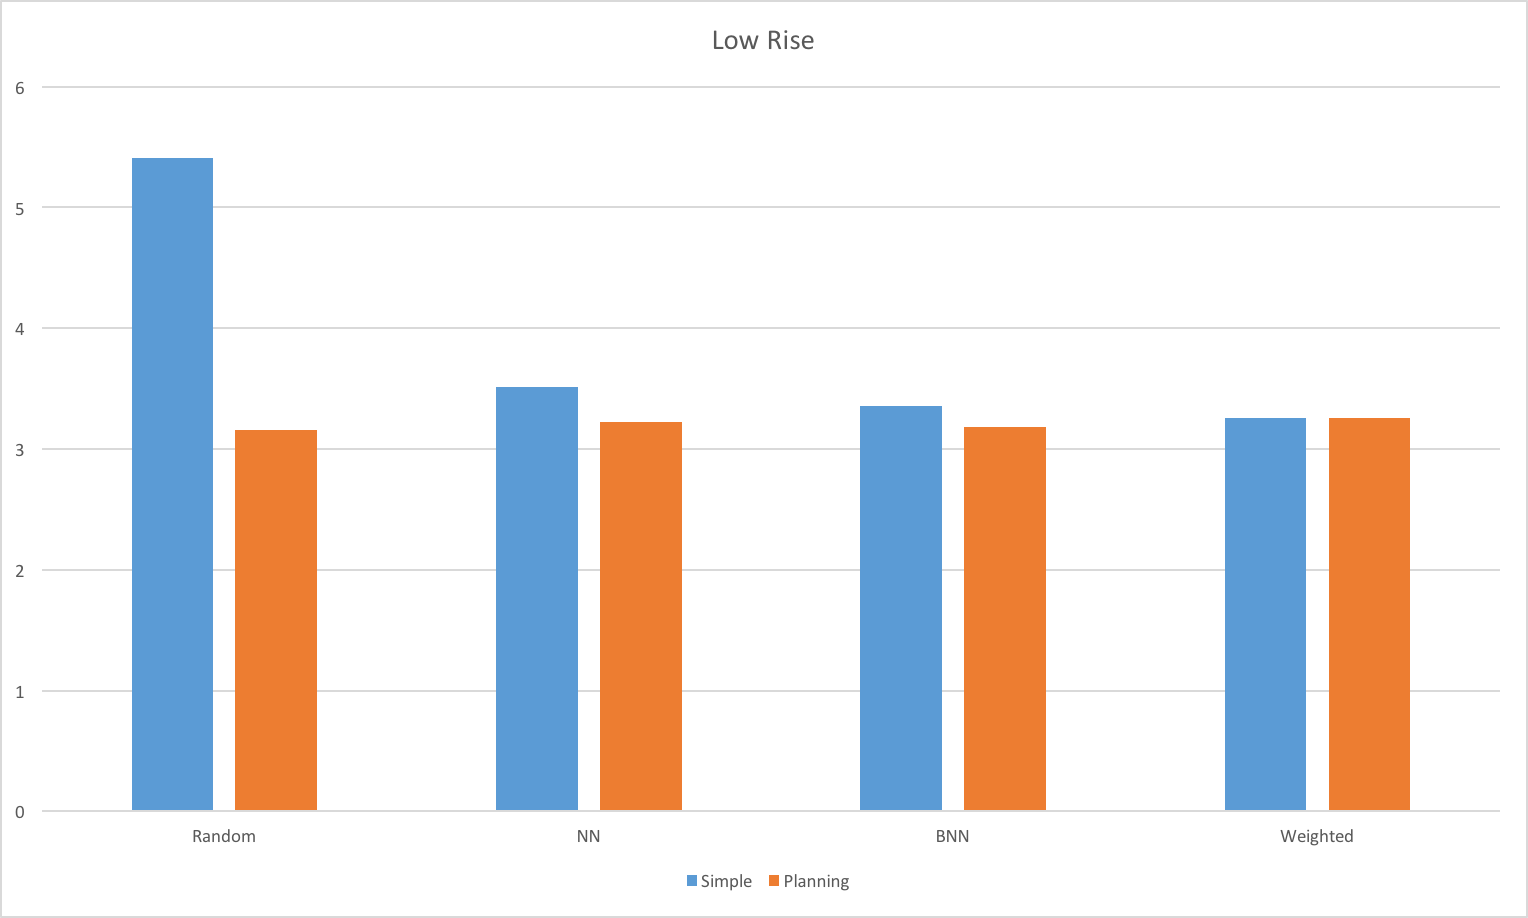
\includegraphics[scale=0.5]{img/chart-averages-low-rise}
  \caption[Tempo médio de espera no cenário \textit{Low-rise}.]{Tempo médio de espera para diferentes estratégias no cenário \textit{Low-rise}.}
  \label{fig:result:average:low-rise}
\end{figure}

\section{Cenário \textit{High-rise}}

\lipsum[1]

\begin{table}[htb!]
\centering
\caption{Parâmetros do cenário \textit{High-rise}.}
\label{tab:results:highrise:params}
\begin{tabular}{|r|l|}
\hline
\textbf{Propriedade}          & \textbf{Valor}       \\ \hline
\textit{Nome}                 & High-rise            \\ \hline
\textit{Duração (s)}          & 43200                \\ \hline
\textit{Semente}              & w9JwgykwejtoL2icSgHo \\ \hline
\textit{Elevadores}           & 8                    \\ \hline
\textit{Capacidade}           & 10                   \\ \hline
\textit{Andares}              & 39                   \\ \hline
\textit{Horizonte (planning)} & 2                    \\ \hline
\end{tabular}
\end{table}

\begin{table}[htb!]
\centering
\caption{Resultados para o cenário \textit{High-rise}.}
\label{tab:results:highrise}
\begin{tabular}{|l|r|r|r|r|r|r|}
\hline
\multicolumn{1}{|c|}{\textbf{}}                 & \multicolumn{3}{c|}{\textbf{Tempo de Espera}}                                                                    & \multicolumn{3}{c|}{\textbf{Tempo de Jornada}}                                                                                                                       \\ \hline
\textbf{Estratégia} & \multicolumn{1}{c|}{\textit{Médio}} & \multicolumn{1}{c|}{\textit{Desvio}} & \multicolumn{1}{c|}{\textit{Total}} & \multicolumn{1}{c|}{\textit{Médio}}                   & \multicolumn{1}{c|}{\textit{Desvio}}                  & \multicolumn{1}{c|}{\textit{Total}}                  \\ \hline
\textit{Simple / Random}          & 25.9981 & 28.0464 & 190124 & 15.2595 & 14.9190 & 111593 \\ \hline
\textit{Simple / NN}              & 20.3395 & 37.1902 & 148743 & 15.0993 & 11.4479 & 110421 \\ \hline
\textit{Simple / BNN}             & 13.5243 & 23.5950 &  98903 & 15.0550 & \cellcolor[HTML]{67FD9A}10.2476 & 110097 \\ \hline
\textit{Simple / Weighted}        & 31.0373 & 54.5909 & 226976 & \cellcolor[HTML]{67FD9A}14.9915 & 18.9700 & \cellcolor[HTML]{67FD9A}109633 \\ \hline
\textit{Planning}                 &  \cellcolor[HTML]{67FD9A}8.6901 & \cellcolor[HTML]{67FD9A}16.2139 &  \cellcolor[HTML]{67FD9A}63551 & 15.1627 & 12.0920 & 110885 \\ \hline
\end{tabular}
\end{table}

\begin{table}[htb]
\centering
\caption{Clientes atendidos no cenário \textit{High-rise}.}
\label{table:results:highrise:clients}
\begin{tabular}{|l|r|r|r|}
\hline
\textbf{Estratégia}        & \multicolumn{1}{l|}{\textbf{Criados}} & \multicolumn{1}{l|}{\textbf{Atendidos}} & \multicolumn{1}{l|}{\textbf{Duração}} \\ \hline
\textit{Simple / Random}   & 7313 & 7313 & 43275 \\ \hline
\textit{Simple / NN}       & 7313 & 7313 & 43334 \\ \hline
\textit{Simple / BNN}      & 7313 & 7313 & 43349 \\ \hline
\textit{Simple / Weighted} & 7313 & 7313 & 43372 \\ \hline
\textit{Planning}          & 7313 & 7313 & 43341 \\ \hline
\end{tabular}
\end{table}

\begin{table}[htb]
\centering
\caption{Tempo de decisão do \textit{planning} no cenário \textit{High-rise}.}
\label{table:results:highrise:time}
\begin{tabular}{|l|r|}
\hline
\textit{Mínimo}  & 0.002097 s \\ \hline
\textit{Mediana} & 0.031623 s \\ \hline
\textit{Média}   & 0.043263 s \\ \hline
\textit{Máximo}  & 0.358810 s \\ \hline
\end{tabular}
\end{table}

\begin{figure}[htb]
  \centering
  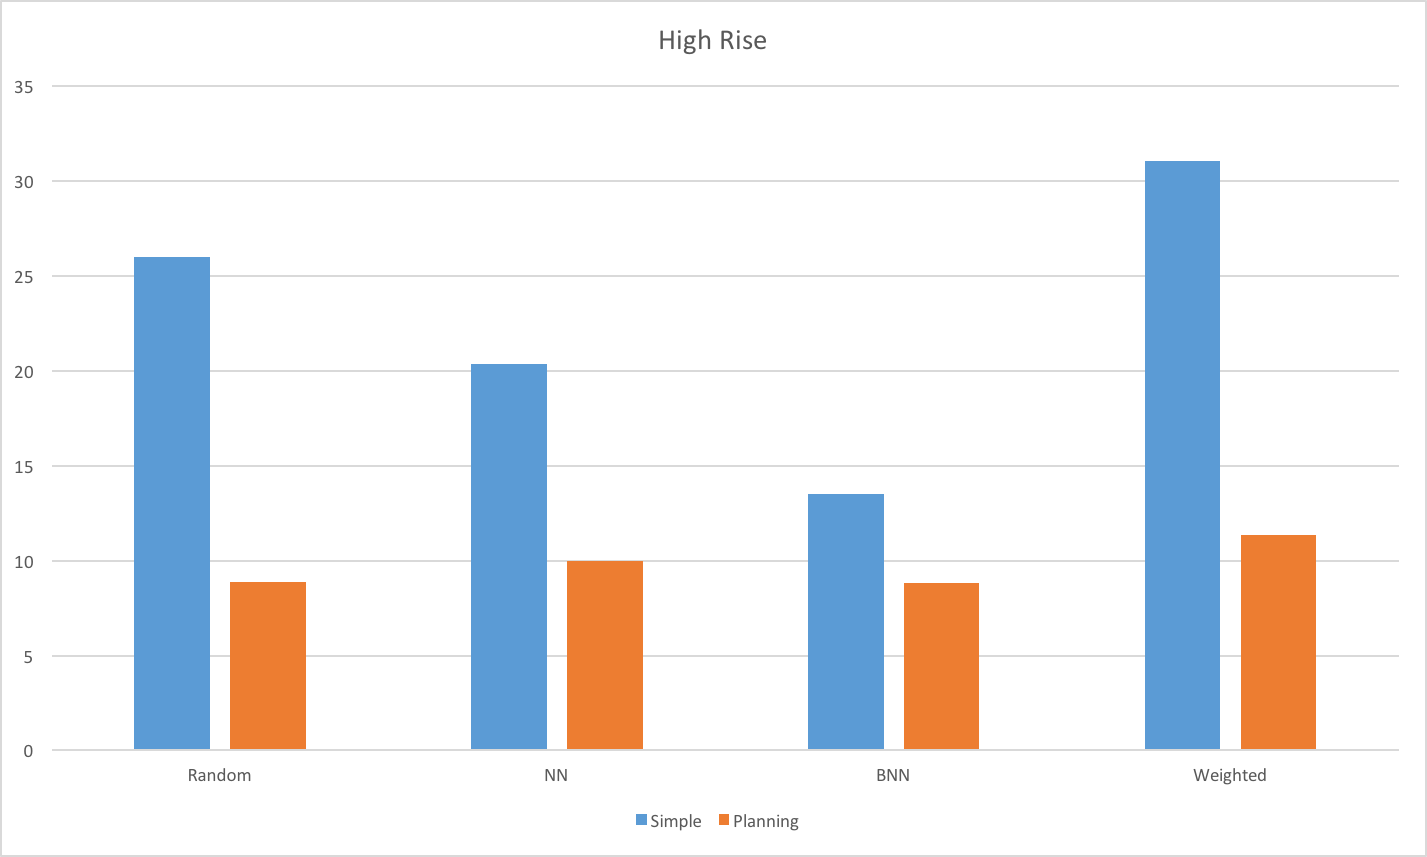
\includegraphics[scale=0.5]{img/chart-averages-high-rise}
  \caption[Tempo médio de espera no cenário \textit{High-rise}.]{Tempo médio de espera para diferentes estratégias no cenário \textit{High-rise}.}
  \label{fig:result:average:high-rise}
\end{figure}

\section{Cenário \textit{Skyscraper}}

\lipsum[1]

\begin{table}[htb!]
\centering
\caption{Parâmetros do cenário \textit{Skyscraper}.}
\label{tab:results:skyscraper:params}
\begin{tabular}{|r|l|}
\hline
\textbf{Propriedade}          & \textbf{Valor}       \\ \hline
\textit{Nome}                 & Skyscraper           \\ \hline
\textit{Duração (s)}          & 43200                \\ \hline
\textit{Semente}              & NimatYvEnU9QeE3GkF4J \\ \hline
\textit{Elevadores}           & 16                   \\ \hline
\textit{Capacidade}           & 12                   \\ \hline
\textit{Andares}              & 163                  \\ \hline
\textit{Horizonte (planning)} & 2                    \\ \hline
\end{tabular}
\end{table}

\begin{table}[htb!]
\centering
\caption{Resultados para o cenário \textit{Skyscraper}.}
\label{tab:results:skyscraper}
\begin{tabular}{|l|r|r|r|r|r|r|}
\hline
\multicolumn{1}{|c|}{\textbf{}}                 & \multicolumn{3}{c|}{\textbf{Tempo de Espera}}                                                                    & \multicolumn{3}{c|}{\textbf{Tempo de Jornada}}                                                                                                                       \\ \hline
\textbf{Estratégia} & \multicolumn{1}{c|}{\textit{Médio}} & \multicolumn{1}{c|}{\textit{Desvio}} & \multicolumn{1}{c|}{\textit{Total}} & \multicolumn{1}{c|}{\textit{Médio}}                   & \multicolumn{1}{c|}{\textit{Desvio}}                  & \multicolumn{1}{c|}{\textit{Total}}                  \\ \hline
\textit{Simple / Random}          & 442.2165 & 1775.3156 & 10538904 & 54.7816 & 389.3520 & 1305554 \\ \hline
\textit{Simple / NN}              & 343.5988 & 1426.3821 &  8188647 & 54.9789 & 291.2258 & 1310258 \\ \hline
\textit{Simple / BNN}             & 287.1803 & 1137.2342 &  6844080 & 55.0124 & 235.4007 & 1311056 \\ \hline
\textit{Simple / Weighted}        & 293.8791 & 1018.5118 &  7003726 & \cellcolor[HTML]{67FD9A}54.6163 & 242.3278 & \cellcolor[HTML]{67FD9A}1301616 \\ \hline
\textit{Planning}                 &  \cellcolor[HTML]{67FD9A}78.3855 &  \cellcolor[HTML]{67FD9A}230.8554 &  \cellcolor[HTML]{67FD9A}1868084 & 60.1728 &  \cellcolor[HTML]{67FD9A}48.8070 & 1434038 \\ \hline
\end{tabular}
\end{table}

\begin{table}[htb]
\centering
\caption{Clientes atendidos no cenário \textit{Skyscraper}.}
\label{table:results:skyscraper:clients}
\begin{tabular}{|l|r|r|r|}
\hline
\textbf{Estratégia}        & \multicolumn{1}{l|}{\textbf{Criados}} & \multicolumn{1}{l|}{\textbf{Atendidos}} & \multicolumn{1}{l|}{\textbf{Duração}} \\ \hline
\textit{Simple / Random}   & 23832 & 23832 & 45037 \\ \hline
\textit{Simple / NN}       & 23832 & 23832 & 45388 \\ \hline
\textit{Simple / BNN}      & 23832 & 23832 & 45131 \\ \hline
\textit{Simple / Weighted} & 23832 & 23832 & 44584 \\ \hline
\textit{Planning}          & 23832 & 23832 & 43688 \\ \hline
\end{tabular}
\end{table}

\begin{table}[htb]
\centering
\caption{Tempo de decisão do \textit{planning} no cenário \textit{Skyscraper}.}
\label{table:results:skyscraper:time}
\begin{tabular}{|l|r|}
\hline
\textit{Mínimo}  & 0.03882 s \\ \hline
\textit{Mediana} & 2.35068 s \\ \hline
\textit{Média}   & 2.12851 s \\ \hline
\textit{Máximo}  & 4.99215 s \\ \hline
\end{tabular}
\end{table}

\begin{figure}[htb]
  \centering
  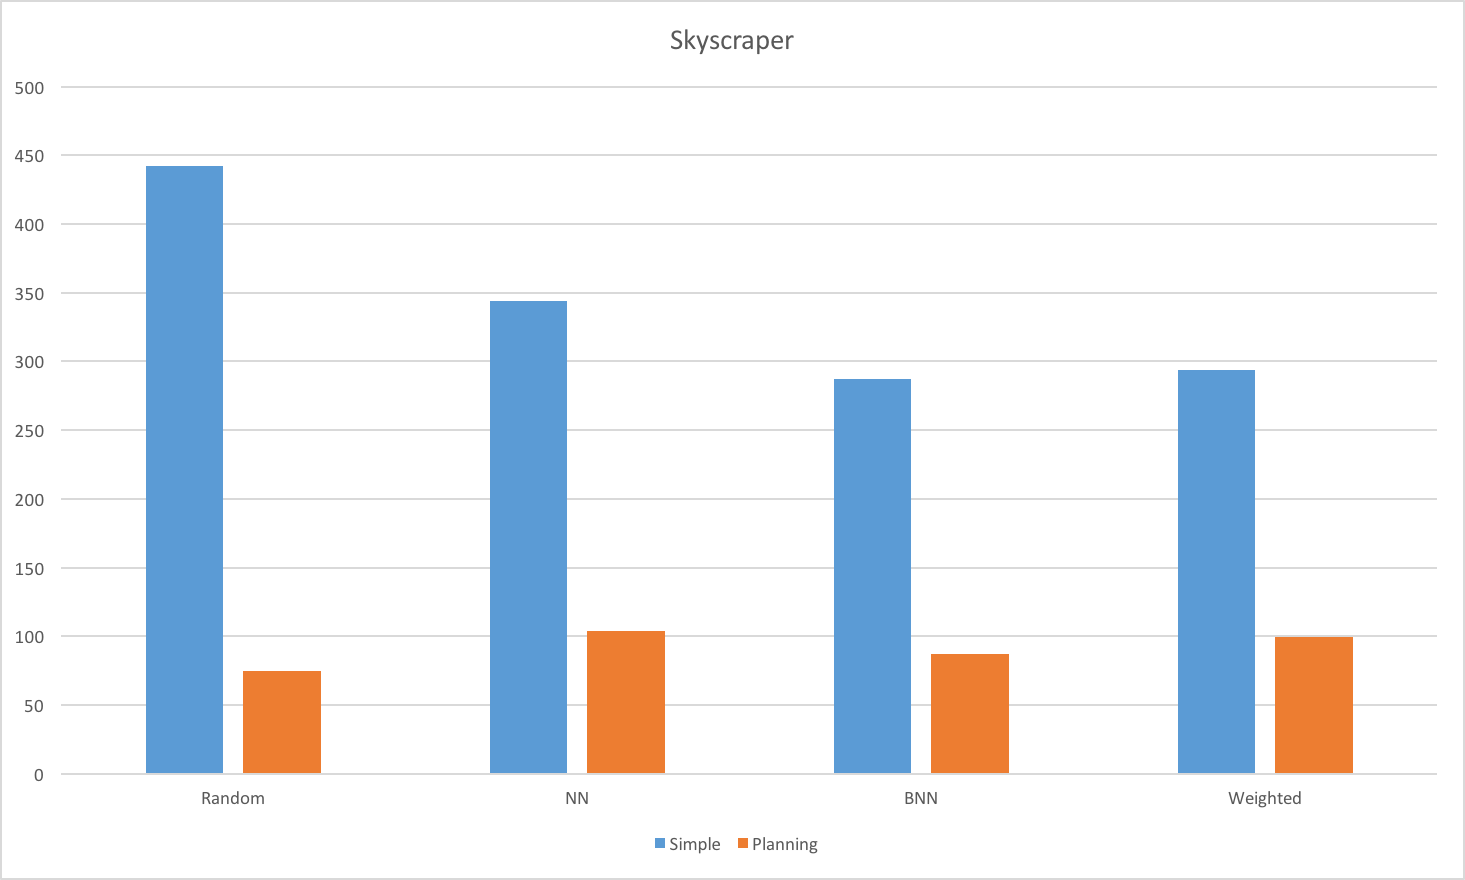
\includegraphics[scale=0.5]{img/chart-averages-skyscraper}
  \caption[{Tempo médio de espera no cenário \textit{Skyscraper}.}]{Tempo médio de espera para diferentes estratégias no cenário \textit{Skyscraper}.}
  \label{fig:result:average:skyscraper}
\end{figure}